\documentclass[12pt]{article}
\usepackage{amsmath}
\usepackage{tikz}
\begin{document}
\title{Computer Science 180, Homework 7}
\date{March 8th, 2018}
\author{Michael Wu\\UID: 404751542}
\maketitle

\section*{Chapter 7, Problem 11}

\begin{center}
        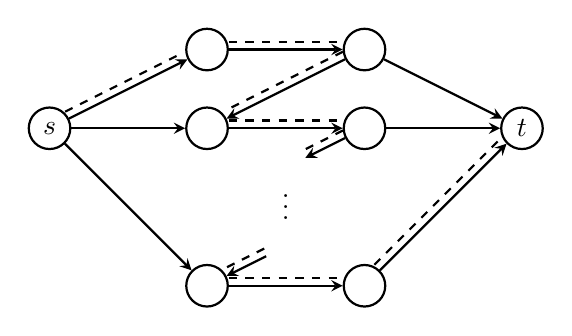
\begin{tikzpicture}
                \begin{scope}[auto, every node/.style={thick, draw,circle,minimum size=1.5em,inner sep=1}, every path/.style={thick, ->, >=stealth}]
                        \node (S) at (0,0) {\(s\)};
                        \node (T) at (6,0) {\(t\)};
                        \node (A) at (2,1) {};
                        \node (B) at (2,0) {};
                        \node (C) at (2,-2) {};
                        \node (D) at (4,1) {};
                        \node (E) at (4,0) {};
                        \node (F) at (4,-2) {};
                        \node [draw=none] (G) at (3,-0.9) {\vdots};
                        \node [draw=none] (H) at (3,-0.5) {};
                        \node [draw=none] (I) at (3,-1.5) {};

                        \path (S) edge (A);
                        \path (S) edge (B);
                        \path (S) edge (C);
                        \path (D) edge (T);
                        \path (E) edge (T);
                        \path (F) edge (T);
                        \path (A) edge (D);
                        \path (B) edge (E);
                        \path (C) edge (F);
                        \path (D) edge (B);
                        \path (E) edge (H);
                        \path (I) edge (C);

               \end{scope}
               \path[thick,dashed,transform canvas={xshift=-0.05cm, yshift=0.0866cm}] (S) edge (A);
               \path[thick,dashed,transform canvas={yshift=0.1cm}] (A) edge (D);
               \path[thick,dashed,transform canvas={xshift=-0.0259cm, yshift=0.0966cm}] (D) edge (B);
               \path[thick,dashed,transform canvas={yshift=0.1cm}] (B) edge (E);
               \path[thick,dashed,transform canvas={xshift=-0.0259cm, yshift=0.0966cm}] (E) edge (H);
               \path[thick,dashed,transform canvas={xshift=-0.0259cm, yshift=0.0966cm}] (I) edge (C);
               \path[thick,dashed,transform canvas={yshift=0.1cm}] (C) edge (F);
               \path[thick,dashed,transform canvas={xshift=-0.0707cm, yshift=0.0707cm}] (F) edge (T);
        \end{tikzpicture}
\end{center}
This statement is false. Consider the graph shown above, where each edge has a capacity of \(1\). There is an arbitrary amount
of rows \(r\) that form paths from the source \(s\) to the sink \(t\), indicated by the vertical dots. Then if the Forward-Edge-Only Algorithm
chooses the path given by the dotted lines, it will terminate with a flow value of \(v(f^\prime)=1\). But
the maximum flow value is \(v(f)=r\), which occurs when every outgoing edge from \(s\) is used. Thus for any constant \(b>1\), we can
create a graph such that the Forward-Edge-Only Algorithm is not guaranteed to find a flow value of at least \(\frac{1}{b}\) times the maximum flow value.
We do this by having \(r>b\) in the graph shown above, then there exists a flow \(f^\prime\) that the Forward-Edge-Only Algorithm can find in this graph where
\[v(f^\prime)=\frac{1}{r}v(f)\]
Thus \(v(f^\prime)\) is \(\frac{1}{r}\) times the maximum flow value, less than \(\frac{1}{b}\) times the maximum flow value.

\pagebreak

\section*{Chapter 7, Problem 14}

\paragraph{a)}

Transform this problem into a network flow problem by creating a source node \(s\) that has an edge \((s,x_i)\) for every node \(x_i\in X\). Then
create a sink node \(t\) and replace every edge into \(S\) with an edge into \(t\). We do not care about edges out of \(S\), as if the flow of people
reaches some node inside \(S\) they are safe and do not need to leave \(S\). We allow multiple edges into \(t\) from a given node \(v\), as this represents
how the node \(v\) may have multiple edges that connect to different nodes \(s_i\in S\). Let the capacity of each edge in our graph be \(1\), representing how
we only allow one group of people to move along an edge. Consolidate multiple edges between two nodes by adding their capacities together. So if there
are three edges from a node \(v\) into \(S\), for example, replace it by an edge \((v,t)\) with capacity \(3\). This transformation gives us a graph
\(G^\prime\) that we can find the maximum flow through in polynomial time using the Ford-Fulkerson algorithm.

If and only if our maximum flow through \(G^\prime\) is equal to \(|X|\), there exists a set of evacuation routes from \(X\) to \(S\) such that no route contains the same edge.
We prove this by noting that if our maximum flow is equal to \(|X|\), then the flow out of \(s\) must pass through every node \(x_i\in X\). This is because
\(s\) has \(|X|\) edges, one to each populated node. Then the path \(P_i=(s,x_i,\ldots,t)\) in \(G^\prime\) has a flow of \(1\) and corresponds to a
path \((x_i,\ldots,s_j)\) for some \(s_j\in S\) that shares no edges with any other evacuation path. So there is a path \(P_i\) for every \(x_i\in X\) that
reaches \(S\) without sharing any edges.

If our maximum flow is less than \(|X|\), no such set of evacuation paths exists. This is because if our maximum flow is less than \(|X|\), this implies there
is an \(s\)-\(t\) cut \((A,B)\) with capacity \(c(A,B)<|X|\). Then only \(c(A,B)\) groups of people can travel into \(B\) while taking unique paths, which
contains the set \(S\subseteq B\). Thus fewer than \(|X|\) groups of people can travel into \(S\) while taking unique paths, and no set of evacuation paths exists where
every populated node has a unique path to \(S\).

\paragraph{b)}

Form \(G^\prime\) as before, except replace each node \(v\) in the original graph \(G\) with \(v_{in}\) and \(v_{out}\). Let there be a single edge \((v_{in},v_{out})\)
with capacity \(1\) in \(G^\prime\). Replace all the incoming edges of the form \((u,v)\) with \((u,v_{in})\) and all the outgoing edges of the form \((v,u)\) with \((v_{out},u)\).
Thus only one group of people can pass through a node in any given path, because only one path can contain the edge \((v_{in},v_{out})\). Otherwise the connections between
our nodes remain the same as in the original graph \(G\). Then as before, we can find the maximum flow through \(G^\prime\) and assert that there exists a set of evacuation routes if and only if the maximum flow is equal to \(|X|\).

A graph \(G\) where this process returns yes for part a) and no for part b) is shown below.

\begin{center}
        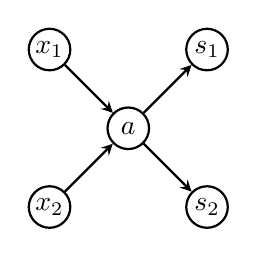
\begin{tikzpicture}
                \begin{scope}[auto, every node/.style={thick, draw,circle,minimum size=1.5em,inner sep=1}, every path/.style={thick, ->, >=stealth}]
                        \node (X2) at (0,0) {\(x_2\)};
                        \node (X1) at (0,2) {\(x_1\)};
                        \node (S2) at (2,0) {\(s_2\)};
                        \node (S1) at (2,2) {\(s_1\)};
                        \node (A) at (1,1) {\(a\)};

                        \path (X1) edge (A);
                        \path (X2) edge (A);
                        \path (A) edge (S1);
                        \path (A) edge (S2);
               \end{scope}
        \end{tikzpicture}
\end{center}
Here \(X=\{x_1,x_2\}\) and \(S=\{s_1, s_2\}\). The corresponding network flow graph \(G^\prime\) for part a) is shown below.
\begin{center}
        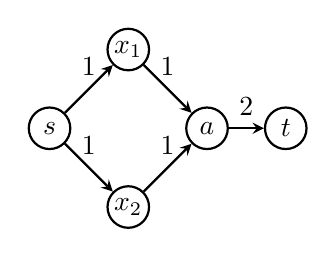
\begin{tikzpicture}
                \begin{scope}[auto, every node/.style={thick, draw,circle,minimum size=1.5em,inner sep=1}, every path/.style={thick, ->, >=stealth}]
                        \node (X2) at (0,0) {\(x_2\)};
                        \node (X1) at (0,2) {\(x_1\)};
                        \node (T) at (2,1) {\(t\)};
                        \node (A) at (1,1) {\(a\)};
                        \node (S) at (-1,1) {\(s\)};

                        \path (X1) edge node[above,draw=none] {1} (A);
                        \path (X2) edge node[above,draw=none] {1} (A);
                        \path (A) edge node[above,draw=none] {2} (T);
                        \path (S) edge node[above,draw=none] {1} (X1);
                        \path (S) edge node[above,draw=none] {1} (X2);
               \end{scope}
        \end{tikzpicture}
\end{center}
This has max flow \(2=|X|\) so our answer is yes. The corresponding network flow graph \(G^\prime\) for part b) is shown below.
\begin{center}
        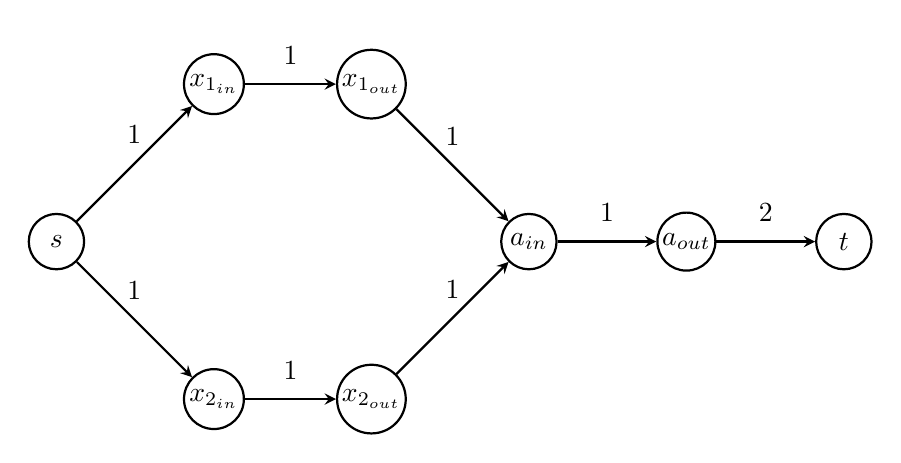
\begin{tikzpicture}
                \begin{scope}[auto, every node/.style={thick, draw,circle,minimum size=2em,inner sep=1}, every path/.style={thick, ->, >=stealth}]
                        \node (X2in) at (-2,0) {\(x_{2_{in}}\)};
                        \node (X1in) at (-2,4) {\(x_{1_{in}}\)};
                        \node (X2out) at (0,0) {\(x_{2_{out}}\)};
                        \node (X1out) at (0,4) {\(x_{1_{out}}\)};
                        \node (T) at (6,2) {\(t\)};
                        \node (Ain) at (2,2) {\(a_{in}\)};
                        \node (Aout) at (4,2) {\(a_{out}\)};
                        \node (S) at (-4,2) {\(s\)};

                        \path (X1out) edge node[above,draw=none] {1} (Ain);
                        \path (X2out) edge node[above,draw=none] {1} (Ain);
                        \path (Aout) edge node[above,draw=none] {2} (T);
                        \path (S) edge node[above,draw=none] {1} (X1in);
                        \path (S) edge node[above,draw=none] {1} (X2in);
                        \path (X1in) edge node[above,draw=none] {1} (X1out);
                        \path (X2in) edge node[above,draw=none] {1} (X2out);
                        \path (Ain) edge node[above,draw=none] {1} (Aout);
               \end{scope}
        \end{tikzpicture}
\end{center}
This has max flow \(1<|X|\) so our answer is no.

\pagebreak

\section*{Chapter 7, Problem 17}

Consider the set \(A\) of points that can be reached from \(s\) after the attack, and the set \(B=V-A\) of points that cannot be reached from \(s\) after
the attack. This forms a minimum cut \((A,B)\), since there are \(k\) removed edges \(e_1,\ldots,e_k\) going out of \(A\) that go into \(B\). Each of these
removed edges \(e_i\) must carry one unit of network flow, because \((A,B)\) is a minimum cut and the capacity of every edge in our graph is \(1\). Then we
can form \(k\) paths \(P_1,\ldots,P_k\) from \(s\) to \(t\) which each represent the flow of one unit of traffic through the network. Let no two paths share
any edges, because if two paths shared an edge \(e\) this would imply that that \(e\) has a capacity greater than \(1\), a contradiction. Furthermore, each
removed edge \(e_i\) from \(A\) to \(B\) must be assigned to a unique path \(P_i\), since each edge \(e_i\) goes from \(A\) to \(B\). If a path does not
contain a removed edge \(e_i\), then it could not go from \(s\in A\) to \(t\in B\). Since each path \(P_i\) contains an edge \(e_i\), and no two paths can share
edges, each path must have one removed edge \(e_i\).

Let \(n\) be the total number of nodes in our graph \(G=(V,E)\). For each path \(P_i\) we can ping \(\log_2(n)\) nodes in \(V\) to find which edge \(e_i\) along
this path was removed by the attacker. This is because the length of \(P_i\) is at most \(n\), and after the path \(P_i\) travels to the first node in \(B\)
no subsequent nodes in \(P_i\) will be reachable. So we can use binary search when pinging to find the removed edge, which has a logarithmic runtime complexity.
So we can find the set of removed edges \(\{e_1,\ldots,e_k\}\) in \(O(k\log n)\) pings, since we run binary search on \(k\) paths. Then
we can simply do a depth first search on the graph \(G^\prime=G-\{e_1,\ldots,e_k\}\) to find \(A\). This requires no pings, as we already know the original graph
\(G\) and the removed edges \(\{e_1,\ldots,e_k\}\). Finally we can return \(B=V-A\) to find the set of nodes not reachable from \(s\).

Although this algorithm requires finding the maximum flow through \(G\), which requires greater than \(O(k\log n)\) time, this step requires no pings. Similarly, no
pings are required to find the paths \(P_1,\ldots,P_k\), as we can construct these solely from our original graph \(G\). So the total amount of pings required grows with
\(O(k\log n)\).

\pagebreak

\section*{Chapter 7, Problem 29}

\end{document}